\lohead{Florian Harrer}

\chapter{Java-Programm}
\label{sec:java-programm}

\section{Anforderungen}
\subsection{Programm}
Die Hauptaufgabe des Programms, welches am Raspberry Pi laufen soll, ist es dem Benutzer eine Möglichkeit zum Steuern der Katzenfütterungsanlage zu Verfügung zu stellen. Weiters soll das Programm die Motoren steuern und die Sensoren in der Anlage auswerten können. Für diese Aufgabe sollen die IO-Pins am Raspberry verwendet werden.
\subsection{Design - Benutzerinterface}
Der Benutzer soll mit Hilfe eines kleinen Touchdisplays die Möglichkeit haben die Anlage zu steuern. Deswegen muss darauf geachtet werden, dass alle GUI-Fenster sinnvoll per Touch-Gesten verwendbar sind.
Das Design der GUI-Fenster soll einfach und übersichtlich gestaltet werden. Auf der Hauptseite, also der Seite die immer zu sehen ist, sollen Informationen dargestellt werden, die dem Benutzer einen schnellen Überblick über den Zustand der Anlage geben. Alle anderen nicht direkt ersichtlichen Funktionen sollen über sinnvoll benamte Menüpunkte erreichbar sein.
\subsection{Externe Steuerung}
Da die Katzenfütterungsanlage die Katze füttern soll, wenn die Familie der Katze auf Urlaub ist, sollte die Anlage auch über das Internet erreichbar sein. Dafür gibt es die Möglichkeit einen Benutzer auf der Anlage anzulegen mit welchem man anschließend über eine Webseite auf die Anlage zugreifen kann. Weiters soll das Java Programm (Server) mit der Web-Applikation (Client) kommunizieren, also Daten austauschen, können.

\newpage

\section{Voruntersuchung}
\subsection{Wieso Java und nicht C?}
Zu Beginn musste entschieden werden mit welcher Programmiersprache gearbeitet werden soll. Zur Auswahl standen Java und C.
Vorteile von C:
\begin{itemize}
\item[1] Programme sind ressourcenschonender
\item[2] Hardwarenahe Programmierung einfach durchführbar, direkter Zugriff auf die Pins
\end{itemize}
Vorteile von Java:
\begin{itemize}
\item[1] Erstellen einer GUI mit Java Swing ist einfacher (weil es im Unterricht erlernt wurde)
\item[2] In Java kann nur sauber programmiert werden (aufgrund der Überprüfung des Compilers)
\end{itemize}

Nach dem Gegenüberstellen der Vorteile wurde Java als Programmiersprache gewählt.

\subsection{Wieso das Raspberry Pi 3 Model B?}
Schon zu Beginn der Diplomarbeit war klar, dass mit deinem Raspberry gearbeitet werden soll. Nun musste entschieden werden welches Model verwendet werden soll.
\\ Technische Daten des Raspberry Pi 3 Model B
\begin{itemize}
\item[1] Rechenleistung (CPU hat 4 Kerne und eine Taktfrequenz von 1,2GHz)
\item[2] Anzahl der GPIO-Pins (26)
\item[3] WLAN-Fähigkeit
\end{itemize}

Technische Daten des Raspberry Pi 3 Model B
\begin{itemize}
\item[1] Rechenleistung (CPU hat 4 Kerne und eine Taktfrequenz von 0,9GHz)
\item[2] Anzahl der GPIO-Pins (26)
\item[3] keine WLAN-Fähigkeit
\end{itemize}

Wir haben das Raspberry Pi 3 Model B, aufgrund der oben angeführten technischen Daten, gewählt. Den größten Einfluss auf die Entscheidung hatte dabei die WLAN-Fähigkeit. Das liegt daran, dass dadurch die Anlage überall im Haus aufgestellt werden kann und keine Ethernetschnittstelle benötigt wird. Ein weiterer positiver Aspekt des Raspberry Pi 3 ist die höhere Rechenleistung.

\subsection{Auswahl eines Touchdisplays}
Das Display muss folgende Anforderungen erfüllen:
\begin{itemize}
\item[1] Es muss ein Touchscreen-Display sein
\item[2] Es muss einfach an das Raspberry anschließbar sein
\item[•] Es soll nicht zu klein sein
\item[3] Es soll nicht zu teuer sein
\end{itemize}

Aufgrund dieser Anforderungen wurde das Touchdisplay von Raspberry gewählt.
\\ Folgende technische Daten des Display legten den Grundstein für die Entscheidung:
\begin{itemize}
\item[•] Das Anschließen des Displays an das Raspberry erfolgt über ein Displayportkabel und zwei Kabel für die Stromversorgung
\item[•] Das Display hat eine Größe von 7 Zoll
\item[•] Der Preis beträgt 70\euro{}
\end{itemize}

\subsection{Wieso pi4j?}
Da Java als Programmiersprache gewählt wurde, musste eine Möglichkeit die GPIO-Pins anzusteuern gefunden werden.
Da bei der Recherche außer pi4j Java kaum etwas gefunden wurde, wurde pi4j gewählt. Weiters vorteilhaft ist, dass das Ansteuern der Pins über die Java Software nicht sehr kompliziert ist. Hierfür müssen nur die Bibliotheken von pi4j in das Projekt eingebunden werden.

\subsection{Wieso Mongodb?}
Eine Datenbank wurde gewählt, weil es gegenüber des Speicherns der Daten in eine Datei mehrere Vorteile aufweist. 
\subsubsection{Vorteil gegenüber Daten in Datei speichern}
Vorteile einer Datenbank:
\begin{itemize}
\item[1] Professionellere Lösung als das Speichern in eine Datei
\item[2] Beim Speichern von großen Datenmengen effizienter
\item[3] Es kann vom Java Programm und vom Webserver zugegriffen werden, ohne dass es zu einem Fehler kommt
\item[4] Das Suchen von Daten ist einfacher
\end{itemize}
\subsubsection{Vergleich mit anderen Datenbanken}
Vergleich von Mongodb mit mySQL:
\begin{itemize}
\item[•] Mongodb
\begin{itemize}
\item[1] Mongodb ist schemenlos und open source
\item[2] Zugriffskonzept basiert auf JSON
\item[3] Benutzern können keine Berechtigungen gegeben/genommen werden
\end{itemize}
\item[•] mySQL
\begin{itemize}
\item[1] mySQL hat ein Datenschema und ist open source
\item[2] Zugriffskonzept auf mehrere Arten
\item[3] Benutzern können Berechtigungen gegeben/genommen werden
\end{itemize}
\end{itemize}

Aufgrund dieser Gründe wurde Mongodb als Datenbank gewählt.

\subsection{Kommunikation mit der Web-Applikation}
Der Server mit dem die Web-Applikation kommunizieren kann, wird aufgrund der gewählten Programmiersprache, in Java geschrieben. Der Server und die Web-Applikation laufen am gleichen System und kommunizieren über einen Socket. Der Server wird im Hintergrund aktiv sein und auf Anfragen der Web-Applikation warten. Je nach Anfrage wird der Server Daten zurück senden oder Methoden im Programm aufrufen. Die Daten, die bei der Kommunikation ausgetauscht werden, haben den Datentyp JSON.

\newpage

\section{Umsetzung}
Bei der Umsetzung, also beim Schreiben des Programms, wurde wie folgt vorgegangen. Zuerst wurden alle GUI-Fenster per Hand grob entworfen. Anschließend wurden diese im Netbeans als javax.swing.JFrame Form erstellt. Genaueres über die GUI-Fenster folgt unter Punkt 2.3.4. Danach wurden grundlegende Funktionen die das Programm zu erfüllen hat implementiert. Weiters wurden noch die Klassen: Mongodb, pi4j, der Server und der ErrorAndWarningHandler als Singleton implementiert. 
\\ \\ 
Nun folgen ausführlichere Beschreibungen über die oben angeführten Klassen.

\subsection{Mongodb}
\subsubsection{Allgemeines}
Mongodb ist ein schemenlose Datenbank. Schemenlos bedeutet, dass die Daten keine besondere Formatierung brauchen um gespeichert zu werden. Zusätzlich wird jedem gespeichertem Datensatz automatisch ein einmaliger Identifikator gegeben. Weiters ist Mongodb open source, das bedeutet, dass es kostenfrei ist.
\\
Bei einer schemenbehafteten Datenbank werden die Daten, in einer Tabelle, in Reihen und Spalten gegliedert. Um eine solche Datenbank effizient nutzen zu können wird ein einmaliger Identifikator verwendet. Dieser verkürzt das Suchen eines Datensatzes.
\\ \\ 
In Mongodb werden die Daten in Collections gespeichert. Die in den Collections gespeicherten Datensätze werden Documents genannt. 
\\ \\
Die Datenbank kann in der Konsole mit dem Befehl \textbf{mongod} gestartet werden. In unserem konkreten Fall am Raspberry startet die Datenbank beim Starten des Raspberry automatisch. Weiters kann in der Konsole mit dem Befehl \textbf{mongo}, sofern die Datenbank gestartet ist, die Mongo-Shell geöffnet werden. In der Shell können alle angelegten Datenbanken verwaltet werden. Unter verwalten wird das Ändern, Hinzufügen und Löschen von Daten verstanden. Es können auch neue Datenbanken angelegt oder alte Datenbanken gelöscht werden. 
\\ Befehle:
\begin{itemize} 
\item[•] \textbf{\inlinecode{JavaStyle}{show dbs}} ... zeigt alle angelegten Datenbanken an
\item[•] \textbf{\inlinecode{JavaStyle}{show collections}} ... zeigt alle collections in einer Datenbank
\item[•] \textbf{\inlinecode{JavaStyle}{use}} ... verwenden einer Datenbank, falls die Datenbank noch nicht existiert wird sie neu erstellt 
\\     (Beispiel: \inlinecode{JavaStyle}{use <Datenbankname>} )
\item[•] \textbf{\inlinecode{JavaStyle}{drop()}} ... löschen einer Datenbank
\\     (Beispiel: \inlinecode{JavaStyle}{<Datenbankname>.drop()} )
\item[•] \textbf{\inlinecode{JavaStyle}{find()}} ... suchen nach bestimmten Daten 
\\     (Beispiel: \inlinecode{JavaStyle}{db.data.find()} )
\item[•] \textbf{\inlinecode{JavaStyle}{count()}} ... zählt die Dokumente in einer Collection
\\     (Beispiel: \inlinecode{JavaStyle}{db.<Collectionname>.count()} )
\item[•] \textbf{\inlinecode{JavaStyle}{insert()}} ... hinzufügen eines Dokumentes
\\     (Beispiel: \inlinecode{JavaStyle}{db.data.insert(\{"time1":"13:30"\}} )
\item[•] \textbf{\inlinecode{JavaStyle}{updateOne()}} ... updaten von Daten
\\     (Beispiel: \inlinecode{JavaStyle}{db.data.updateOne(<DokumentID>, <Daten>)} )
\item[•] \textbf{\inlinecode{JavaStyle}{deleteOne()}} ... löschen eins Dokumentes
\\     (Beispiel: \inlinecode{JavaStyle}{db.data.deleteOne(<DokumentID>)} )
\end{itemize}

\subsubsection{Datenbankmanagementsystem DBMS}
Ein Datenbankmanagementsystem verwaltet eine oder mehrere Datenbanken. Mehrere Datenbanken werden dabei benötigt, wenn mehrere Anwendungen oder Programme jeweils eine eigene Datenbank brauchen. Ein Beispiel für ein DBMS ist Mongodb.

\subsubsection{Singleton}
Der Datenbankzugriff wurde in einem Singleton implementiert. Dadurch wird nur ein Objekt der Datenbank erzeugt. Das bedeutet, dass nur von diesem Objekt aus auf die Datenbank zugegriffen wird und nur eine Verbindung geöffnet wird.
\\ Ein weiterer Vorteil davon ist, dass wenn einmal eine andere Datenbank verwendet werden sollte, nur diese eine Klasse geändert werden muss, weil nur in dieser Klasse der Code für die spezifische Datenbank enthalten ist. Diese Art von Klasse nennt man Wrapper-Klasse. Das bedeutet, dass diese Klasse einen Teil des Codes des Programms beinhaltet, welcher nur in dieser Klasse vorkommt.

\subsubsection{Code Beispiele}
Da am Raspberry die neueste Version von Mongodb nicht funktioniert, wird die Version 2.14.2 verwendet. Weitere Details zu diesem Thema sind unter Punkt 2.4.1 zu finden.
\\ Aus diesem Grund sind auch die Methoden, die als Beispiele angeführt sind, von der älteren Version. 
\\ \\ 
Als Erstes muss eine Verbindung mit der Datenbank aufgebaut werden. Falls die Datenbank noch nicht existiert wird sie automatisch erstellt.
Dies ist in Java mit folgenden Methoden möglich:
\begin{lstlisting}[style=JavaStyle, caption=Mit Mongodb verbinden]
	MongoClient mongodb = new MongoClient();
	DB database = mongodb.getDB("<Datenbankname>");
\end{lstlisting}

Danach muss die Collection, in der gearbeitet werden soll, ausgewählt werden. Falls die Collection noch nicht existiert wird sie automatisch erstellt. Das ist mit der folgenden Methode möglich:
\begin{lstlisting}[style=JavaStyle, caption=Collection auswählen]
	DBCollection coll = database.getCollection("<Collectionname>");
\end{lstlisting}
Anschließend kann mit der Datenbank gearbeitet werden. 
\begin{itemize}
\item[•] Die Dokumente in einer Collection zählen:
\begin{lstlisting}[style=JavaStyle, caption=Anzahl der Collections zählen]
	<Collectionname>.count();
\end{lstlisting}
\item[•] Ein Dokument aus der Datenbank lesen:
\begin{lstlisting}[style=JavaStyle, caption=Nach Dokument suchen]
	DBObject document = <Collectionname>.find(<Identifikator>).next();
\end{lstlisting}
\item[•] Ein Dokument zu einer Collection hinzufügen:
\begin{lstlisting}[style=JavaStyle, caption=Ein Dokument hinzufügen]
	<Collectionname>.insert(document);
\end{lstlisting}	
\item[•] Ein Dokument in einer Collection updaten:
\begin{lstlisting}[style=JavaStyle, caption=Ein Dokument updaten]
	<Collectionname>.update(<Identifikator>, document);
\end{lstlisting}
\end{itemize}

Bevor das Java Programm beendet wird sollte die Verbindung zur Datenbank wie folgt getrennt werden: 
\begin{lstlisting}[style=JavaStyle, caption=Verbindung zur Datenbank trennen]
	mongodb.close();
\end{lstlisting}

Ein konkretes Beispiel des Codes aus dem Programm für die Katzenfütterungsanlage sieht so aus:
\begin{lstlisting}[style=JavaStyle, caption=Konkretes Beispiel: Dokument suchen, label=BspDokumentSuchen]
	DBObject document = collUser.find(
			new BasicDBObject("identifier", "User")).next();
\end{lstlisting}
Im Code-Beispiel \ref{BspDokumentSuchen} wird in der Collection \textbf{collUser} nach dem Dokument mit dem Identifikator \textbf{\inlinecode{JavaStyle}{new BasicDBObject("identifier", "User")}} gesucht. Das gefundene Dokument wird dann dem \textbf{DBObject document} zugewiesen. 


\subsection{pi4j} \label{subsec:pi4j}
\subsubsection{Allgemeines}
Pi4j ist eine open source Software, welche Bibliotheken zur Verfügung stellt, mit denen es möglich ist, von einem Java Programm, wenn es auf einem Raspberry ausgeführt wird, auf die IO-Pins dess Raspberrys zuzugreifen. Dabei kann ein GPIO-Pin als In- oder Ouput definiert werden. Wenn ein Pin als Output definiert wird, kann er den Zustand High (+3,3V) oder Low (0V) haben. Mit einem Input Pin, können digitale Signale gemessen werden. Das Ergebnis der Messung ist wieder High oder Low. Weiters ist es auch möglich einem Pin einen Listener zuzuweisen. Dieser Listener wartet bis auf diesem Pin ein Event auftritt und führt dann zum Beispiel eine Methode aus. 
\\ \\

\begin{wrapfigure}{l}{0.5\textwidth}
\vspace{-35pt}
  \begin{center}
    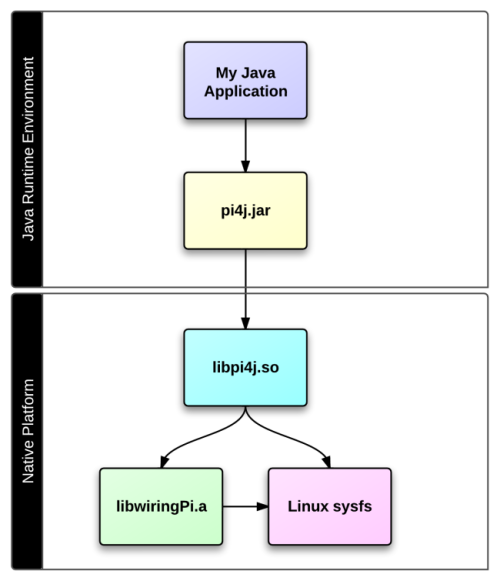
\includegraphics[width=0.45\textwidth]{Bilder/pi4j/dependencies}
  \end{center}
  \caption[Abhängigkeiten]{Abhängigkeiten\protect\footnotemark}
  \label{Abhaengigkeiten}
  \vspace{-160pt}
\end{wrapfigure}

\footnotetext{\autoref{Abhaengigkeiten} Quelle: \url{http://pi4j.com/dependency.html} (besucht am: 02/03/2018)}

Pi4j stellt mithilfe des JNI (Java Native Interface) eine Verbindung von der JVM (Java Virtual Machine) zu dem nativen System des Raspberys her. Dadurch wird es möglich ist zu sehen, wie vom Java-Programm auf die Pins zugefriffen wird.
\\ Der konkrete Zugriff erfolgt über die Bibliothek \textbf{libwiringPi}.


\newpage

\subsubsection{Pin Numbering Sheme}

\begin{wrapfigure}{l}{0.5\textwidth}
\vspace{-35pt}
  \begin{center}
    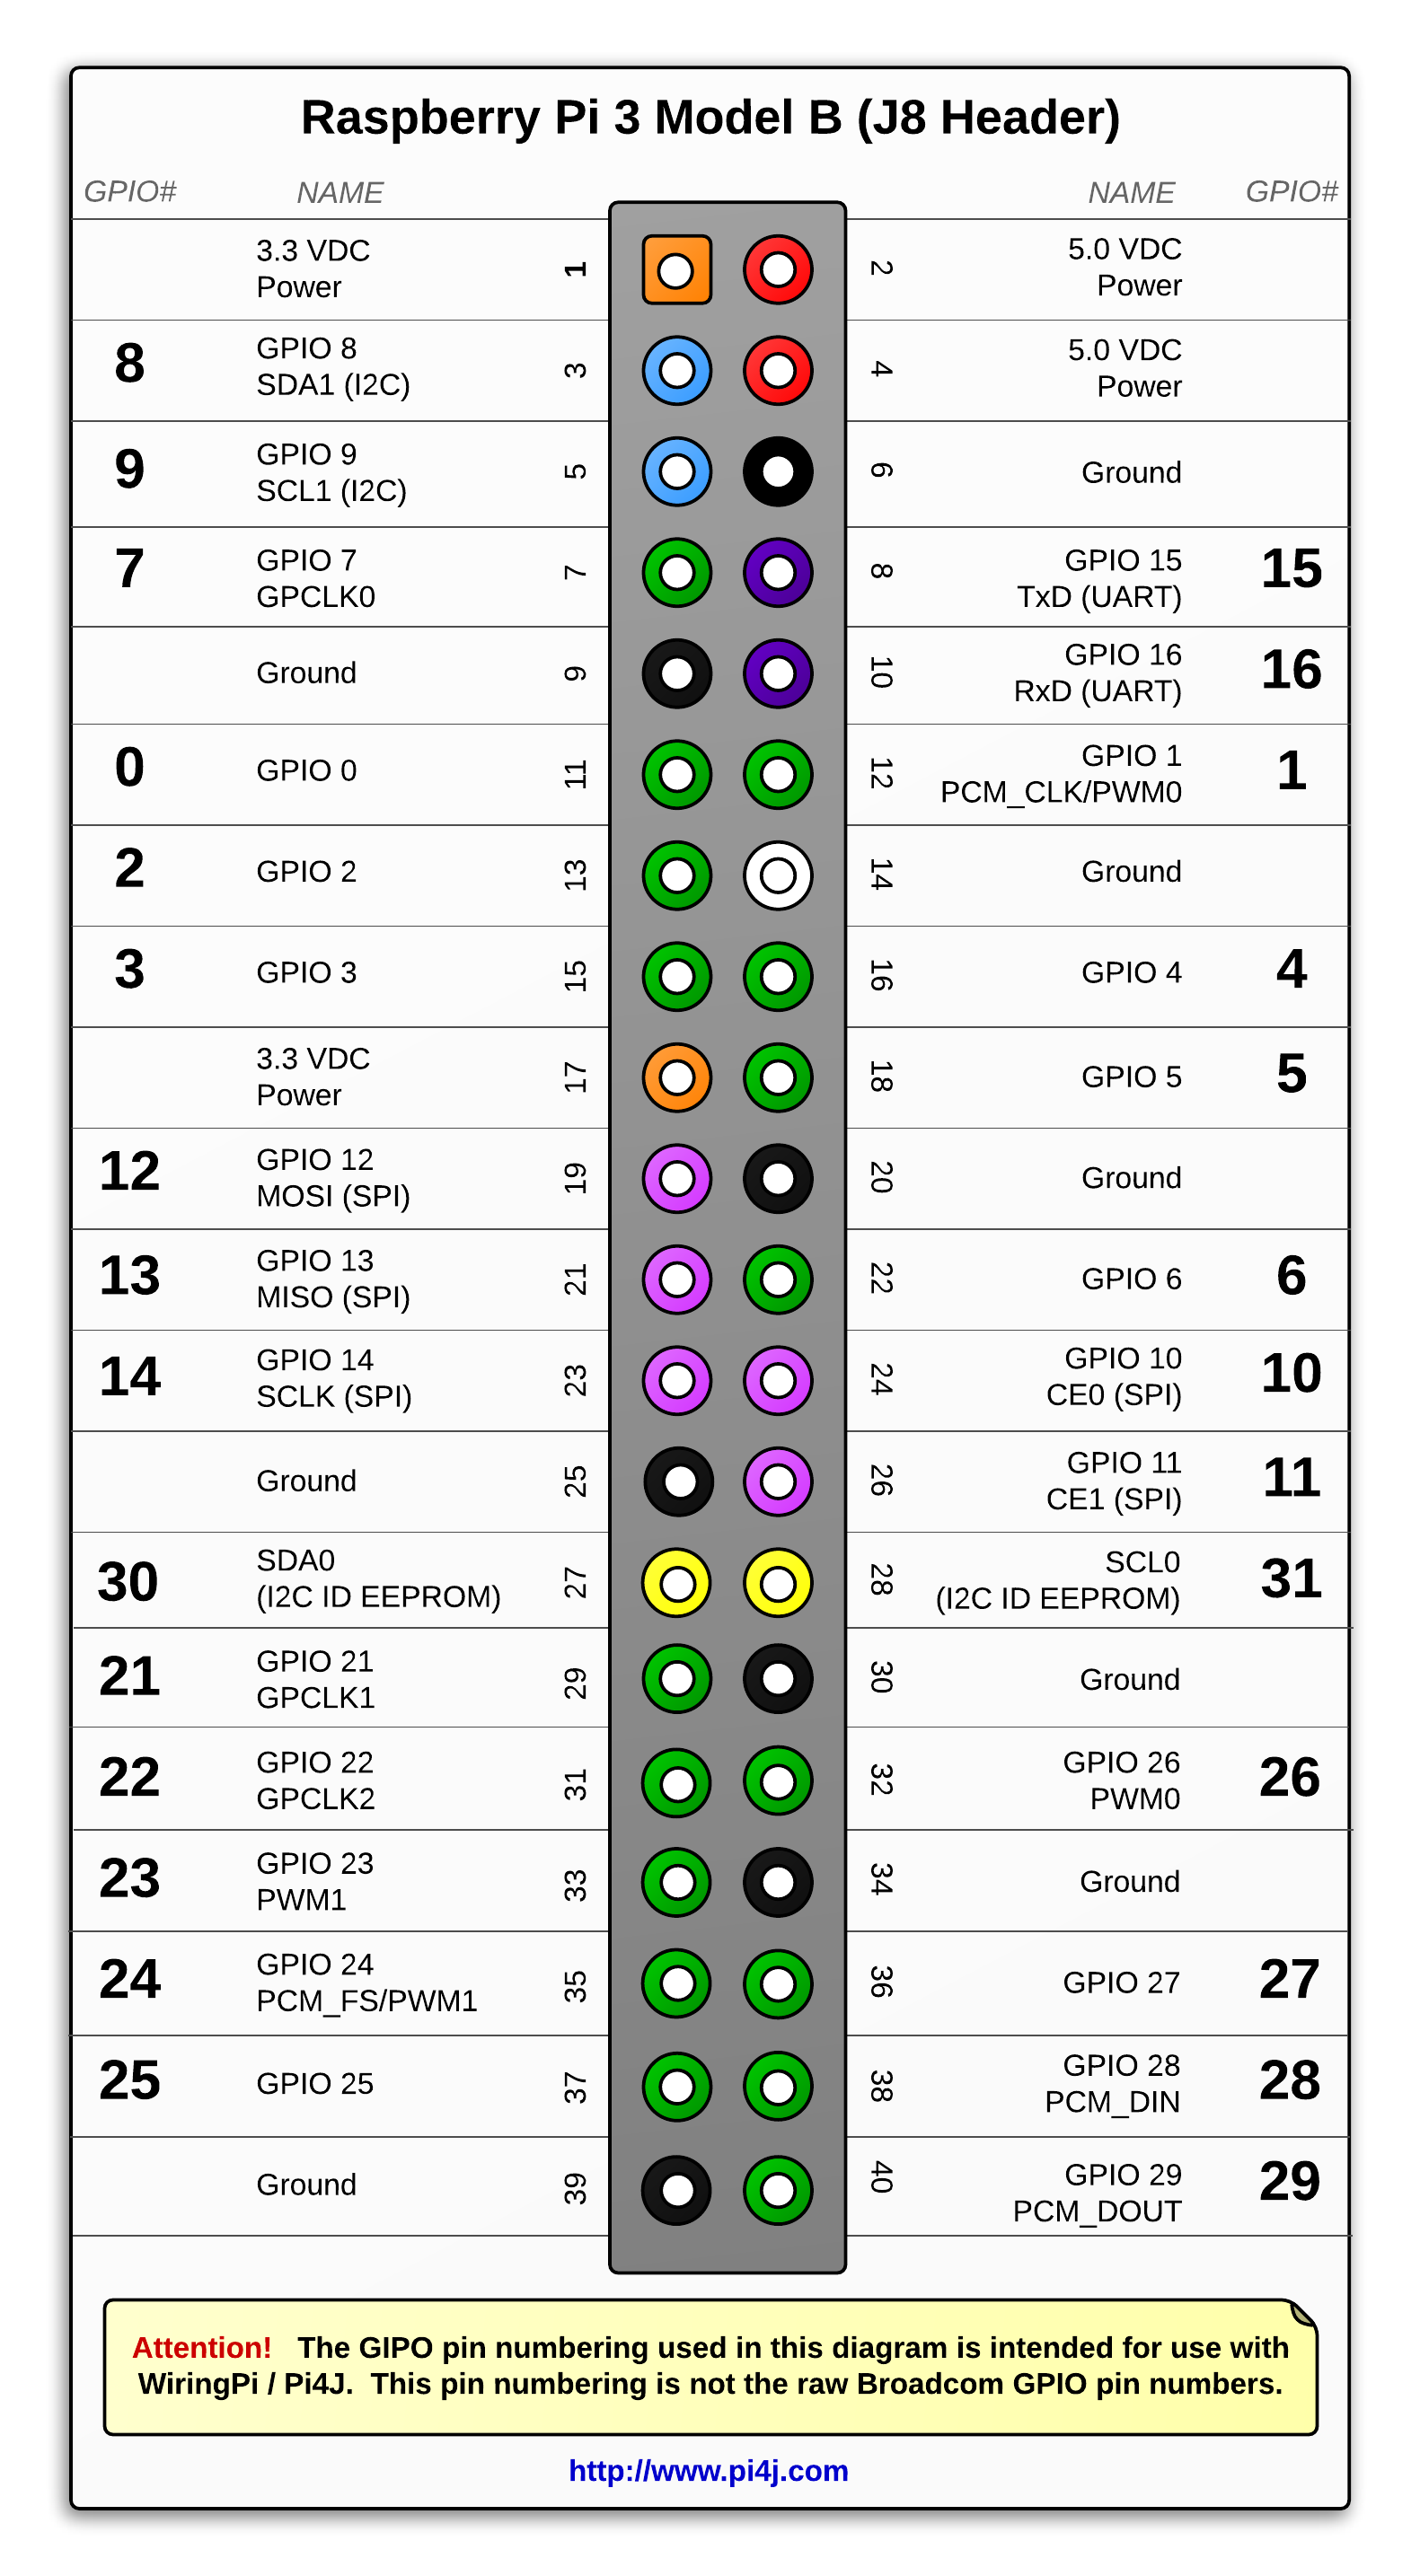
\includegraphics[width=0.50\textwidth]{Bilder/pi4j/PinNumberingSheme}
  \end{center}
  \caption[Pin Numbering Sheme]{Pin Numbering Sheme\protect\footnotemark}
  \label{Pin Numbering Sheme}
  \vspace{-160pt}
\end{wrapfigure}

\footnotetext{\autoref{Pin Numbering Sheme} Quelle: \url{http://pi4j.com/pins/model-3b-rev1.html} (besucht am: 02/03/2018)}

In der Abbildung \ref{Pin Numbering Sheme} ist zu sehen wie die Pins bei einem Raspberry Pi 3 Model B belegt sind.
\\ \\
Am Raspberry haben einige Pins schon fest zugewiesene Funktionen, aber bei den 29 GPIO-Pins kann der Programmierer selbst entscheiden, welche Funktion der Pin wahrnehmen soll.
\\Pins auf die über die mit pi4j nicht zugegriffen werden kann sind:
\begin{itemize}
\item[•] Power mit 3,3V oder 5V
\item[•] Ground
\end{itemize}
\vspace{10pt}
Auch unter den GPIO-Pins gibt es Pins mit einer zusätzlichen Funktion. Zum Beispiel können der GPIO-Pin 15 und 16 für eine UART-Übertragung genutzt werden. Die GPIO-Pins 12, 13 und 14 dienen als SPI Schnittstelle.

\vspace{120pt}

\subsubsection{Gewählte Pin Belegung}
Zum Ansteuern der Motoren und Auswerten der Sensoren wurden nur GPIO-Pins verwendet. Die Motoren in der Anlage werden über jeweils eine H-Brücke angesteuert. Das bedeutet, dass jeder der zwei Motoren jeweils mit vier Transistoren angesteuert wird. Jeder Transistor wird von einem eigenen Pin angesteuert. Für die Sensoren wird jeweils ein Pin zum Auswerten benötigt. In Summe werden zehn GPIO-Pins benötigt. 

\newpage

Diese GPIO-Pins werden, wie folgenden Tabelle 2.1 veranschaulicht, verwendet:

\begin{table}[htb]
\centering
\begin{tabular}{|l|l|}
\hline
\textbf{Pin} & \textbf{Verwendungszweck}          \\ \hline
GPIO\_00     & Sensor Schüsselplatte              \\ \hline
GPIO\_01     & Sensor Förderband (Futtersackerl)  \\ \hline
GPIO\_02     & Motor Schüsselplatte: Aktivieren \\ \hline
GPIO\_03     & Motor Schüsselplatte: Drehen im Uhrzeigersinn \\ \hline
GPIO\_04     & Motor Schüsselplatte: Drehen gegen den Uhrzeigersinn \\ \hline
GPIO\_06     & Motor Förderband: Aktivieren     \\ \hline
GPIO\_10     & Motor Förderband: Drehen im Uhrzeigersinn     \\ \hline
GPIO\_08     & Motor Förderband: Drehen gegen den Uhrzeigersinn     \\ \hline
\end{tabular}
\caption{Belegung der GPIO-Pins}
\label{Pinbelegung}
\end{table}

Wenn einer der beiden Sensoren betätigt wird, liefert dieser das Signal High (+3,3V). Wenn der Sensor nicht betätigt ist liefert dieser Low (0V). 
\\ Um einen Motor einzuschalten müssen jeweils zwei GPIO-Pins auf High geschalten werden. Zuerst muss der Motor aktiviert werden. Wenn der Motor nicht aktiviert ist, ist er ausgeschalten und vom Stromnetz getrennt. Weiters muss dann noch ein weiterer GPIO-Pin auf High geschalten werden. Dieser weitere Pin gibt die Drehrichtung des Motors an. 

\vspace{10pt}

\begin{table}[htb]
\scriptsize
\centering
\caption{Signalverlauf}
\label{Signalverlauf}
\begin{tabular}{|c|c|c|c|c|}
\hline
Motor/Sensor                           & Signal am Motor/Sensor & Zustand des Motors/Sensors              & GPIO-Pin Nummer                                                        & Signal am GPIO-Pin                                        \\ \hline
\multirow{2}{*}{Sensor Schüsselplatte} & High                   & betätigt                                & GPIO\_00                                                               & High                                                      \\ \cline{2-5} 
                                       & Low                    & nicht betätigt                          & GPIO\_00                                                               & Low                                                       \\ \hline
\multirow{2}{*}{Sensor Förderband}     & High                   & betätigt                                & GPIO\_01                                                               & High                                                      \\ \cline{2-5} 
                                       & Low                    & nicht betätigt                          & GPIO\_01                                                               & Low                                                       \\ \hline
\multirow{4}{*}{Motor Schüsselplatte}  & Low                    & steht still, Stromversorung deaktiviert & \begin{tabular}[c]{@{}c@{}}GPIO\_02\\ GPIO\_03\\ GPIO\_04\end{tabular} & \begin{tabular}[c]{@{}c@{}}Low\\ Low\\ Low\end{tabular}   \\ \cline{2-5} 
                                       & Low                    & steht still, Stromversorung aktiviert   & \begin{tabular}[c]{@{}c@{}}GPIO\_02\\ GPIO\_03\\ GPIO\_04\end{tabular} & \begin{tabular}[c]{@{}c@{}}High\\ Low\\ Low\end{tabular}  \\ \cline{2-5} 
                                       & High                   & Motor dreht im Uhrzeigersinn            & \begin{tabular}[c]{@{}c@{}}GPIO\_02\\ GPIO\_03\\ GPIO\_04\end{tabular} & \begin{tabular}[c]{@{}c@{}}High\\ High\\ Low\end{tabular} \\ \cline{2-5} 
                                       & High                   & Motor dreht gegen Uhrzeigersinm         & \begin{tabular}[c]{@{}c@{}}GPIO\_02\\ GPIO\_03\\ GPIO\_04\end{tabular} & \begin{tabular}[c]{@{}c@{}}High\\ Low\\ High\end{tabular} \\ \hline
\multirow{4}{*}{Motor Förderband}      & Low                    & steht still, Stromversorung deaktiviert & \begin{tabular}[c]{@{}c@{}}GPIO\_06\\ GPIO\_10\\ GPIO\_08\end{tabular} & \begin{tabular}[c]{@{}c@{}}Low\\ Low\\ Low\end{tabular}   \\ \cline{2-5} 
                                       & Low                    & steht still, Stromversorung aktiviert   & \begin{tabular}[c]{@{}c@{}}GPIO\_06\\ GPIO\_10\\ GPIO\_08\end{tabular} & \begin{tabular}[c]{@{}c@{}}High\\ Low\\ Low\end{tabular}  \\ \cline{2-5} 
                                       & High                   & Motor dreht im Uhrzeigersinm            & \begin{tabular}[c]{@{}c@{}}GPIO\_06\\ GPIO\_10\\ GPIO\_08\end{tabular} & \begin{tabular}[c]{@{}c@{}}High\\ High\\ Low\end{tabular} \\ \cline{2-5} 
                                       & High                   & Motor dreht gegen Uhrzeigersinm         & \begin{tabular}[c]{@{}c@{}}GPIO\_06\\ GPIO\_10\\ GPIO\_08\end{tabular} & \begin{tabular}[c]{@{}c@{}}High\\ Low\\ High\end{tabular} \\ \hline
\end{tabular}
\end{table}

\vspace{10pt}

Die GPIO-Pins des Raspberrys werden nicht direkt mit den Motoren und Sensoren verbunden. Die GPIO-Pins werden mit einer Treiberstufe verbunden. Diese Treiberstufe steuert direkt die Motoren und holt die Signale von den Sensoren und gibt sie an den Raspberry weiter.

\subsubsection{Singleton}
Die benötigten Methoden von pi4j wurden in einer Wrapper-Klasse als Singleton implementiert. Es wird ein Singleton verwendet, weil der benötigte Controller für die Pins nur einmal erzeugt werden kann. Wenn der Controller trotzdem öfters erzeugt wird, wird  eine Exception geworfen. Der Singleton wird nun dazu verwendet, dass auf die Pins von unterschiedlichen Klassen zugegriffen werden kann.

\subsubsection{Code Beispiele}
Um mit den GPIO-Pins arbeiten zu können muss zu Beginn ein Controller erstellt werden. Dies ist wie folgt möglich:
\begin{lstlisting}[style=JavaStyle, caption=GPIO-Controller erstellen]
	GpioController controller = com.pi4j.io.gpio.GpioFactory.getInstance();
\end{lstlisting}
Wenn der Controller erstellt ist kann auf die Pins, mit denen gearbeitet werden soll, zugegriffen werden. Bei einem Pin kann auch eine \textbf{ShutDownOption} angeben werden. Diese gibt an in welchen Zustand der Pin vor dem Herunterfahren gesetzt wird. Dieser Zugriff erfolgt wie folgt: 
\begin{itemize}
\item[•] Zugreigen auf einen Pin als digitalen Input-Pin:
\begin{lstlisting}[style=JavaStyle, caption=Zugriff auf einen Pin als Inpput]
	GpioPinDigitalInput pin = controller.provisionDigitalInputPin(
		RaspiPin.GPIO_00, PinPullResistance.PULL_DOWN);
	pin.setShutdownOptions(true);
\end{lstlisting}
\item[•] Zugreigen auf einen Pin als digitalen Output-Pin:
\begin{lstlisting}[style=JavaStyle, caption=Zugriff auf einen Pin als Output]
	GpioPinDigitalOutput pin = controller.provisionDigitalOutputPin(
		RaspiPin.GPIO_02, PinState.LOW);
	pin.setShutdownOptions(true, PinState.LOW);
\end{lstlisting}
\end{itemize}
Wenn das erledigt ist kann mit dem Pin gearbeitet werden. Dies kann wie in den folgenden Beispielen erfolgen:
\begin{itemize}
\item[•] Zustand eines Input-Pins auswerten: 
\begin{lstlisting}[style=JavaStyle, caption=Pinzustand abfragen]
	pin.getState()
\end{lstlisting}
Diese Methode liefert den Zustand des Pins zurück. Dieser kann High oder Low sein.

\newpage

\item[•] Zustand eines Output-Pins setzen:
\begin{lstlisting}[style=JavaStyle, caption=Pinzustand verändern]
	pin.low();	
	pin.high();
\end{lstlisting}
Mit \textbf{pin.low()} kann der Zustand eines Pins auf Low (0V) und mit \textbf{pin.high()} auf High (+5V) gesetzt werden. 
\end{itemize}

Vor dem Beenden des Java Programmes sollte der Controller wie folgt heruntergefahren werden:
\begin{lstlisting}[style=JavaStyle, caption=Controller herunterfahren]
	controller.shutdown();
\end{lstlisting}

\subsection{Server-Client-Kommunikation}
\subsubsection{Server}
Der Server wird beim Starten des Java Programmes mithilfe des SwingWorkers in einem eigenen Hintergrund-Thread gestartet. In diesem Hintergrund-Thread wartet der Server bis ein Client versucht Kontakt mit ihm aufzunehmen. Wenn die Verbindung akzeptiert wird, wird ein neuer Thread geöffnet in dem die Kommunikation mit diesem Client abläuft. Sobald die Kommunikation beendet ist wird der zuvor geöffnete Thread wieder geschlossen. 
\\ Der Server wurde auch als Singleton implementiert damit von anderen Klassen einfach auf ihn zugegriffen werden kann.

\subsubsection{Übertragungsprotokoll}
Im Übertragungsprotokoll wird festgelegt wie die Kommunikation zwischen Server und Client abläuft. Hier wird festgelegt was ein gültige Request (Anfrage) ist und wie die Response (Antwort) auf den jeweiligen Request aussieht. Weiters wird festgelegt auf welchen Technologien die Kommunikation basiert. Zusätzlich wird noch der Verbindungsaufbau sowie der Abbau beschrieben.
\\ \\
Die Kommunikation zwischen Server und Client basiert bei der Katzenfütterungsanlage auf Sockets. Diese Sockets basieren auf TCP. Dies ist ein verbindungsorientiertes Protokoll. Das bedeutet, dass Pakete automatisch erneut geschickt werden, wenn bei der Übertragung ein Fehler passiert ist oder das Paket verloren gegangen ist. Der Verbingungsaufbau und Abbau erfolgt bei diesem Protokoll über das IDLE-RQ Verfahren.
\\ Als Timeout wurden 10 Sekunden gewählt, weil das sinnvoll zu sein scheint.
\\ \\
Wenn der Request des Clients mit einem \textbf{GET} beginnt, bedeutet das, dass der Client Daten vom Server fordert. Beginnt der Request mit einem \textbf{PUT}, bedeutet das, dass der Client dem Server Daten schicken will.
\\ Nach jedem \textbf{GET} oder \textbf{PUT} folgt ein Befehl der angibt, welche Daten der Client fordert oder welche Daten der Client dem Server schicken will.
\\ \\
Die folgende Tabelle zeigt alle gültigen Requests und die jeweilige Response darauf:

\begin{table}[htb]
\centering
\begin{tabular}{|l|l|p{300pt}|}
\hline
\multicolumn{2}{|c|}{\textbf{Request}}                                    & \multicolumn{1}{c|}{\multirow{2}{*}{\textbf{Response}}}                                          \\ \cline{1-2}
\multicolumn{1}{|c|}{\textbf{Aktion}} & \multicolumn{1}{c|}{\textbf{Befehl}} & \multicolumn{1}{c|}{}                                                                            \\ \hline
GET                                   & /errors\_warnings                 & Der Server schickt dem Client die aktuell anzuzeigenden Errors und Warnungen in einer Json-Array \\ \hline
PUT                                   & /ChangeMachineState               & Der Server ruft eine Methode auf um den Maschinenzustand zu ändern                               \\ \hline
\end{tabular}
\caption{Übertragungsprotokoll}
\label{Übertragungsprotokoll}
\end{table}

\subsubsection{Response-GET}
Wenn der Server einen Request mit dem Beginn \textbf{GET} bekommt, muss er dem Client die Daten schicken. 
\\ Bei der Katzenfütterungsanlage werden dem Client vom Server die ganzen auftretenten Errors und Warnungen geschickt. Die Errors und Warnungen werdem dem Client als Json-Array geschickt. Diese Json-Array wird in der Klasse, welche alle Errors and Warnungen verarbeitet, erstellt. Die Json-Array ist unter Punkt \ref{subsubsec:Array} dargestellt. 

\subsubsection{Response-PUT}
Wenn der Server einen Request mit dem Beginn \textbf{PUT} bekommt, muss er Daten vom Client entgegen nehmen.
\\ Bei der Katzenfütterungsanlage bekommt der Server die Daten nicht direkt. Da der Maschinenzustand nur \textbf{Ein} oder \textbf{Aus} sein kann, wird dieser nicht übermittelt. Stattdessen wird, wenn der Request zum Ändern des Maschinenzustands erhalten wird, die Methode \textbf{machineStateChanger()} aufgerufen, welche den Maschinenzustand ändert. Diese Methode aktualisiert auch die GUI-Elemente am Raspberry, abhängig vom Maschinenzustand. 

\subsubsection{Verarbeiten des Requests}
Um den Request zu verarbeiten wurde die Klasse \textbf{ConnectionThread} geschrieben. Der Request wird wie folgt verarbeitet:
\begin{itemize}
\item[1] Der Request wird eingelesen.
\item[2] Danach wird überprüft, ob der Request "GET\grqq{} oder "PUT\grqq{} enthält. Wenn keine dieser beiden Funktionen enthalten ist, wird eine Fehlermeldung gesendet.
\item[3] Wenn dies überprüft wurde und kein Fehler aufgetreten ist, wird der Befehl überprüft. Über den Befehl erfährt der Server was er machen soll. Der Inhalt des Befehls ist ein String und wird im Übertragungsprotokoll festgelegt.
\end{itemize}

\subsection{Errors und Warnungsverarbeitung}
\subsubsection{Allgemeines}
Der Benutzer der Katzenfütterungsanlage muss über Fehler, die während des Programmablaufs auftreten, informiert werden. 
\\ Dazu dient die \textbf{ErrorAndWarningHandler} welcher in einer Wrapper-Klasse als Singleton implementiert wurde. In dieser Klasse ist für jeden möglichen Fehler eine Boolean Variable angelegt. Beim Auftreten eines Fehlers wird die zum Fehler gehörende Boolean Variable auf \textbf{true} gesetzt. Beim Erstellen der Liste, die die Errors und Warnungen enthält, werden die jeweiligen Boolean-Variablen abgefragt. Wenn die Boolean-Variable \textbf{true} ist, wird der Error oder die Warnung hinzugefügt. 

\subsubsection{Errors und Warnungen aktivieren/deaktivieren}
Um die Boolean-Variable, die die Errors and Warnungen aktiviert, auf true zu setzen, muss die jeweils zum Error oder zur Warnung gehörende Methode aufgerufen werden. Diese Methode kann wie folgt aussehen:
\begin{lstlisting}[style=JavaStyle, caption=Error setzen]
public void setFeedingHasFailedError (Boolean errorOn)
    {
        error_hasFeedingFailed = errorOn;
        if (errorOn == true)
        {
            failedFeedingTime = String.format("%1$tH:%1$tM", 
            	new Date(System.currentTimeMillis()));
        }   
    }
\end{lstlisting}
In diesem konkreten Beispiel wird der Error, der dem Benutzer mitteilt, dass eine Fütterung fehlgeschlagen hat, aktiviert. Mit dem Parameter \textbf{errorOn} kann bestimmt werden, ob der Error aktiv oder inaktiv sein soll. Wenn der Parameter \textbf{true} ist, ist der Error aktiv. Daraus folgt, dass der Error inaktiv ist, wenn \textbf{errorOn = false} ist. 
\\ In dieser Methode wird zusätzlich ein Zeitstempel erstellt. Dieser Zeitstempel wird nur erstellt, wenn der Error aktiviert wird. 

\subsubsection{Json-Array} \label{subsubsec:Array}
Diese Klasse stellt auch die Json-Array zur Verfügung, welche dann dem Client (Web-Applikation) geschickt wird. 

Die JsonArray kann wie folgt aussehen, wenn Errors sowie auch Warnungen enthalten sind:

\begin{lstlisting}[language=json,firstnumber=1, caption=Json-Objekt mit Errors und Warnungen]
{ 
	"Errors": 
	[ 
		{"message" : "Error1", "hidden" : false}, 
		{"message" : "Error2", "hidden" : false} 
	] 
	"Warnings": 
	[ 
		{"message" : "Warning1", "hidden" : false}, 
		{"message" : "Warning2", "hidden" : false} 
	] 
} 
\end{lstlisting}

\begin{comment} % auskommentiert, weil es wahrschienlich weggenommen wird
\subsubsection{Listenmodel}
Die Zeile, in der die Klasse für das Listenmodel angelegt wird, sieht wie folgt aus:
\begin{lstlisting}[style=JavaStyle, caption=Listenmodel-Klasse erstellen]
	public class ErrorAndWarningModel extends AbstractListModel<String>
\end{lstlisting}
Nach dem Klassennamen muss \textbf{extends AbstractListModel} hinzugefügt werden. Dies bedeutet, dass das erstellte Listemodel von \textbf{AbstractListModel} abgeleitet ist.
\\ \\
Das Listenmodel wird wie folgt angelegt:
\begin{lstlisting}[style=JavaStyle, caption=Liste erstellen im Model]
	private final List<String> errorAndWarning;
\end{lstlisting}
Damit ist nun festgelegt, dass die Elemente in der Liste Strings sind. 

\subsubsection{Liste}
Eine Liste in Java wird dazu verwendet, um mehrere Daten in einem Objekt zu speichern. Die Liste kann wie folgt erstellt werden:
\begin{lstlisting}[style=JavaStyle, caption=Liste erstellen]
	List<String> list = new ArrayList<>();
\end{lstlisting}
Das Objekt der Liste verfügt über eigene Methoden. 
\begin{itemize}
\item[•] Anzahl der Elemente in der Liste zählen: 
\begin{lstlisting}[style=JavaStyle, caption=Anzahl der Elemente abfragen]
	list.size();
\end{lstlisting}
\item[•] Hinzufügen eines Elementes:
\begin{lstlisting}[style=JavaStyle, caption=Element hinzufügen]
	list.add("Das ist ein Element!");
\end{lstlisting}
\item[•] Leeren der Liste (Löschen aller Elemente)
\begin{lstlisting}[style=JavaStyle, caption=Liste leeren]
	list.clear();
\end{lstlisting}
\end{itemize}

Die Errors und Warnungen, die in der Liste gespeichert werden, werden in der GUI in einer Liste (jList) dargestellt. Siehe Kapitel \ref{subsubsec:MainWindow}. 
\end{comment}  % kommentar ende

\subsection{SwingWorker}
Der SwingWorker in Java wird benötigt, wenn eine Methode mehr Zeit benötigt und somit die GUI blockieren würde. Mithilfe des SwingWorkers, aus der Klasse javax.swing, kann diese Aktion in einem Hintergrund-Thread ausgeführt werden. Der Vorteil davon ist, dass die GUI bedienbar bleibt und nicht blockiert. Dafür wird dann mit Hilfe des SwingWorkers ein Hintergrund-Thread geöffnet in dem die Aktion, die mehr Zeit benötigt, abgearbeitet wird.
\\ \\
Das oben geführte Beispiel könnte auch mit der Klasse Thread gelöst werden. Der Hauptgrund für die Verwendung von SwingWorker ist, dass der SwingWorker für die Verwenung in Applikationen mit GUI optimiert ist. Der SwingWorker verfügt über Methoden mit denen nach oder während des Ablaufens des Hintergrundprozzes auf die GUI-Elemente zugegriffen werden kann.
\\ \\ 
Um den SwingWorker verwenden zu können, muss die Klasse wie folgt erstellt werden:
\begin{lstlisting}[style=JavaStyle, caption=SwingWorker Klasse erstellen]
	private class Worker extends SwingWorker<Object, String> { } 
\end{lstlisting}
Im Generic steht als Erstes der Rückgabewert von \textbf{get()} und als Zweites der Datentyp des Übergabewertes von \textbf{publish()}.

\newpage

\subsubsection{EDT}
Im \ac{EDT} wird der Quellcode sequentiell abgearbeitet. Dies bedeutet, dass alle Methoden ihre benötigte Zeit in Anspruch nehmen und danach die jeweils Nächste ausgeführt wird. Im Grunde wird dann ein SwingWorker verwendet, wenn die GUI für den Benutzer merklich blockiert. In der Regel wird gesagt, dass dann ein SwingWorker verwendet werden soll, wenn die Möglichkeit besteht, dass die GUI für 100 Millisekunden oder mehr blockiert.

\subsubsection{TimeUnit}
Wenn ein Hintergrund-Thread mit einer \textbf{while() Schleife} implementiert ist, wiederholen sich die Methoden in der Schleife nach jedem Durchgang wieder. Wenn dies ohne ein Warten passiert, wird sehr viel Prozessorleistung benötigt. \\ Deswegen wird die Methode \inlinecode{JavaStyle}{TimeUnit.MILLISECONDS.sleep(500);} verwendet. Mit dieser Methode wartet das Programm für 500 Millisekunden, ohne Rechenleistung zu konsumieren. Dadurch wird der Prozessor nicht so stark ausgelastet. 

\subsubsection{Methoden des SwingWorkers}
\begin{itemize}
\item[•] doInBackground()
\\ Mit \textbf{doInBackground()} wird ein neuer Hintergrund-Thread erstellt. Dieser Thread läuft parallel zum \ac{EDT}. Der Hintergrund-Thread wird geschlossen, wenn der SwingWorker mit \inlinecode{JavaStyle}{.cancel()} beendet wird oder sich der SwingWorker selbst beendet, weil er alle Methoden abgearbeitet hat. In einem Hintergrund-Thread darf nicht auf die GUI-Elemente von javax.swing.JFrame zugegriffen werden. 
\\ Im folgenden Beispiel wird ein Hintergrund-Thread gezeigt, welcher durch das Beenden des SwingWorkers mit \inlinecode{JavaStyle}{.cancel()} beendbar ist.
\begin{lstlisting}[style=JavaStyle, caption=SwingWorker \inlinecode{JavaStyle}{doInBackground()} mit while Schleife]
	    @Override
        protected Object doInBackground() throws Exception
        {
            while (!isCancelled())
            {
                timeOfDay = String.format("%1$tH:%1$tM", new
                Date(System.currentTimeMillis()));

                publish( timeOfDay);

                TimeUnit.MILLISECONDS.sleep(500);
            }
            return 1;
        }
\end{lstlisting} 
Wenn der SwingWorker beendet wird, während wegen der Methode \\ \inlinecode{JavaStyle}{TimeUnit.MILLISECONDS.sleep(500);} gewartet wird, wird eine \textbf{InterruptedException} geworfen.

\vspace{10pt}

Folgender Hintergrund-Thread arbeitet die Methoden nur einmal ab und wird dann beendet. 
\begin{lstlisting}[style=JavaStyle, caption=SwingWorker \inlinecode{JavaStyle}{doInBackground()} ohne while Schleife, label=SwingWorkerOhneWhileSchleife]
	    @Override
        protected String doInBackground() throws Exception
        {
            String timeOfDay = String.format("%1$tH:%1$tM", new 
            Date(System.currentTimeMillis()));
            
            return timeOfDay;
        }
\end{lstlisting} 

\item[•] done()
\\ Wenn ein Hintergrund-Thread beendet wird, wird \textbf{done()} im EDT aufgerufen. Im \textbf{done()} können dann GUI-Elemente bearbeitet werden. Wenn das Code-Beispiel \ref{SwingWorkerOhneWhileSchleife} als Beispiel herangezogen wird könnte die \textbf{done()} wie folgt aussehen:
\begin{lstlisting}[style=JavaStyle, caption=SwingWorker done()]
	    @Override
        protected void done()
        {
             String time = get();
        }
\end{lstlisting}
\item[•] process()
\\ Wenn in einem Hintergrund-Thread \textbf{publish();} aufgerufen wird, wird im EDT \textbf{process()} aufgerufen. Hier können wieder GUI-Elemente bearbeitet werden.
\begin{lstlisting}[style=JavaStyle, caption=SwingWorker process()]
        @Override
        protected void process(List<String[]> chunks)
        {
            String[] chunk = chunks.get((chunks.size() - 1));
            
            lbTimeOfDay.setText(chunk[0]);
            lbDate.setText(chunk[2]);
        }
\end{lstlisting}

\newpage

\item[•] cancel()
\\ Mit \inlinecode{JavaStyle}{.cancel()} kann ein SwingWorker beendet werden. Dafür muss folgender Befehl aufgerufen werden:
\begin{lstlisting}[style=JavaStyle, caption=SwingWorker abbrechen]
	    worker.cancel();
\end{lstlisting}
Bei diesem Methodenaufruf ist \textbf{worker} die Objektvariable des SwingWorkers.
\end{itemize}

\subsection{GUI-Fenster}
Die GUI-Fenster stellen die grafische Oberfläche für den Benutzer zur Verfügung. Da ein Touchscreen-Display verwendet wird, ist es möglich alle GUI-Fenster mit berühren des Touchscreens, mit einem Finger, zu bedienen. 
\\ Beim Starten des Raspberrys wird das Programm automatisch gestartet. Dabei wird das MainWindow, also das Hauptfenster des Programms, als Vollbild am Display angezeigt. Somit ist es dem Benutzer nur möglich das Programm zu bedienen und nicht zur grafischen Oberfläche des Raspberrybetriebsystems zu gelangen. Genaueres zum Autostart unter Kapitel \ref{subsubsec:Autostart}.

\subsubsection{Java-Programm im Autostart}\label{subsubsec:Autostart}
Um auf einem Bietriebssystem, dass auf Linux basiert, ein Java-Programm zu starten gibt es zwei Möglichkeiten.
\begin{itemize}
\item[1] \textbf{rc.local}
\\ Eine Möglichkeit ist die \textbf{rc.local}. Mit der \textbf{rc.local} können aber nur Programme ohne grafische Oberfläche gestartet werden. In diese muss folgender Befehl geschrieben werden: 
\\ \textbf{java -jar /home/pi/main.jar \&}.
\item[2] \textbf{autostart}
\\ Dies zweite Möglichkeit ist \textbf{autostart}. Hier ist der X-Server, welcher für eine grafische Ausgabe benötigt wird, bereits aktiv. Somit können nun Java-Programme mit einer grafischen Oberfläche gestartet werden. Die Datei \textbf{autostart} ist unter folgendem Pfad zu finden : 
\\ \textbf{/home/<user/.config/lxsession/LXDE-<user>/autostart}. 
\\ In die Datei muss dann noch folgender Befehl eingegeben werden: 
\\ \textbf{@java -jar /home/pi/main.jar \&}.
\\Das \textbf{@} am Beginn der Zeile sagt aus, dass das Programm, wenn es nicht ordnungsgemäß geschlossen wird, automatisch neu geöffnet wird.
\end{itemize} 
Bei beiden Möglichkeiten wird jeweils \textbf{main.jar} als Programm angegeben. Dies stellt im Fall eines Programms mit GUI das Hauptfenster dar. Bei der Katzenfütterungsanlage ist es das \textbf{MainWindow}.
\\ \\ Die Abkürzung \textbf{.jar} steht für "Java Archive".

\newpage

\subsubsection{MainWindow}\label{subsubsec:MainWindow}
\begin{wrapfigure}{l}{0.6\textwidth}
\vspace{-20pt}
  \begin{center}
    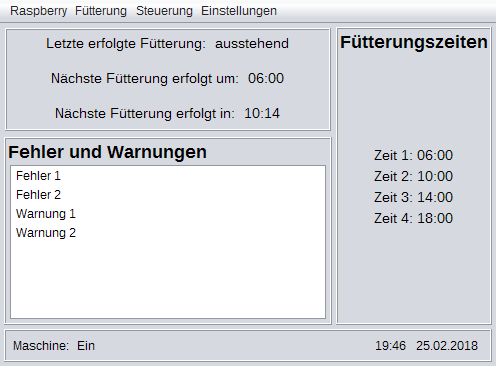
\includegraphics[width=0.60\textwidth]{Bilder/GUI/MainWindow}
  \end{center}
  \caption{MainWindow}
  \label{MainWindow}
  \vspace{20pt}
\end{wrapfigure}
Das \textbf{MainWindow} besteht aus einer \textbf{javax.swing.JFrame Form}. In diesem Fenster wird dem Benutzer ein allgemeiner Überblick über die Anlage zur Verfügung gestellt. Somit können alle wichtigen Informationen schnell und leicht ersichtlich. Weiters ist das \textbf{MainWindow} das Hauptfenster des Programms. Über diese sind alle Dialog-, Steuerungs- und Informationsfenster erreichbar. Diese Fenster werden von Kapitel\ref{TimeManagement} bis Kapitel \ref{Update} genauer beschrieben. Das Aufrufen von anderen Fenstern ist über die Menüleiste, welche sich oben in der GUI befindet, möglich. 
\\ \\ Unter den Menüs der Menüleiste sind folgende Menüpunkte zu finden:
\begin{itemize}
\item[1] Raspberry
\begin{itemize}
\item[•] Neustarten
\item[•] Herunterfahren
\end{itemize}
\item[2] Fütterung
\begin{itemize}
\item[•] Einschalten/Ausschalten
\item[•] Fütterungszeiten verwalten
\end{itemize}
\item[3] Steuerung
\begin{itemize}
\item[•] manuelle Steuerung
\item[•] Positionsinformation
\end{itemize}
\item[4] Einstellungen
\begin{itemize}
\item[•] Update
\item[•] Benutzer anlegen
\item[•] WLAN
\item[•] Geräteinformation
\end{itemize}
\end{itemize}

\vspace{10pt}

Das \textbf{MainWindow} ist als Singleton implementiert, weil dadurch nicht jedes mal, wenn eine andere Klasse auf ein Datenelement des \textbf{MainWindow} zugreift, ein neues Objekt von \textbf{MainWindow} erzeugt wird. Somit wird ein nur Objekt des \textbf{MainWindow} erstellt. Das Singleton-Objekt wurde wie folgt erstellt:
\begin{lstlisting}[style=JavaStyle, caption=MainWindow createInstance()]
public static MainWindow createInstance()
    {
        if (instance != null)
        {
            throw new RuntimeException("intance already created");
        }

        if (!SwingUtilities.isEventDispatchThread())
        {
            throw new RuntimeException("not in EDT");
        }
        instance = new MainWindow();

        return instance;
    }
\end{lstlisting}
Diese Methode kann nur im EDT aufgerufen werden. Wenn diese Methode nicht im EDT aufgerufen wird oder das Objekt bereits besteht, wird eine jeweils eigene Exception geworfen.
\\ \\ Diese Methode wird in der \textbf{main} Methode der Klasse wie folgt aufgerufen:
\begin{lstlisting}[style=JavaStyle, caption=MainWindow createInstance() Aufruf]
	java.awt.EventQueue.invokeLater(new Runnable()
        {
            @Override
            public void run()
            {
                MainWindow frame = MainWindow.createInstance();

            }
        });
\end{lstlisting}

\newpage

Bis jetzt wurde der Singleton nur implementiert. Nun muss noch eine Methode implementiert werden um die \textbf{Instance} des Objekts abfragen zu können. Diese Methode sieht wie folgt aus:
\begin{lstlisting}[style=JavaStyle, caption=MainWindow.getInstance()]
public static MainWindow getInstance()
    {
        if (instance == null)
        {
            throw new RuntimeException("instance not created");
        }

        return instance;
    }
\end{lstlisting}

\vspace{10pt}

In der GUI werden je nach Maschinenstatus gewisse Funktionen blockiert. Folgende Funktionen sind blockiert, wenn die Fütterung aktiviert ist:
\begin{itemize}
\item[1] manuelle Steuerung
\item[2] Update
\end{itemize}
Das Blockieren das Funktionen wird mit folgender Methode gemacht:
\begin{lstlisting}[style=JavaStyle, caption=GUI Elemente blockieren]
private void updateGUIElements()
    {
        // control GUI elements depending on the machine state
        // update and manualControl not available while machine state = on 
        if (machineStateOn == true)
        {
            menuUpdate.setEnabled(false);
            menuManualControl.setEnabled(false);
        }
        else
        {
            menuUpdate.setEnabled(true);
            menuManualControl.setEnabled(true);
        }
    }
\end{lstlisting}

\newpage

\subsubsection{TimeManagement}\label{subsubsec:TimeManagement}
\begin{wrapfigure}{l}{0.65\textwidth}
\vspace{-20pt}
  \begin{center}
    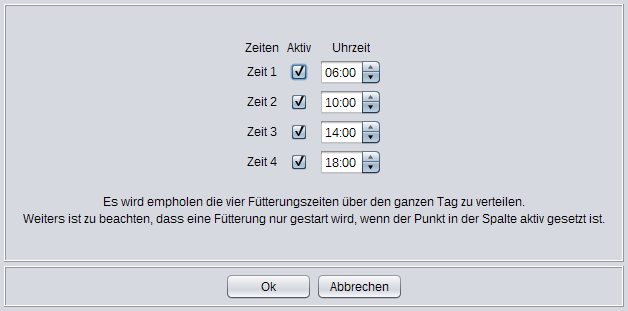
\includegraphics[width=0.65\textwidth]{Bilder/GUI/TimeManagement}
  \end{center}
  \caption{TimeManagement}
  \label{TimeManagement}
  \vspace{0pt}
\end{wrapfigure}
In der Klasse \textbf{TimeManagement} ist es dem Benutzer möglich alle Zeiten zu verwalten. Das GUI-Fenster dieser Klasse ist ein Dialogfenster. Bei Dialogfenstern ist es üblich, dass sie mit \textbf{Ok} und \textbf{Abbrechen} bedienbar sind.
\\ \\ Es können bis zu vier verschiedene Zeiten gewählt werden. Dabei müssen die Zeiten, bei Zeit 1 beginnend, aufsteigend angeordnet werden. Zusätzlich können Zeiten auch deaktiviert werden. Um eine Zeit zu deaktivieren muss das Häkchen vor der Zeit weggenommen werden.
\\ Wenn die Zeiten ausgewählt wurden, kann mit \textbf{Ok} bestätigt werden. Somit werden die Daten in das Programm übernommen und in die Datenbank gespeichert. Weiters schließt sich noch das Fenster.
\\ Falls \textbf{Abbrechen} gedrückt wird, werden die Änderungen nicht übernommen und das Fenster schließt sich.
\\ \\ Wenn das Dialogfenster im EDT aufgerufen wird, blockiert der EDT an dieser Stelle so lange, bis das Dialogfenster wieder geschlossen wird.

\vspace{10pt}

Es sind nur vier Fütterungen pro Tag möglich, weil die Katzenfütterungsanlage ein kleines Futtermagazin hat. Aus diesem Grund würde das Magazin bei mehreren Fütterungen sehr schnell leeren. Wenn das nun passiert erfüllt die Katzenfütterungsanlage ihren Zweck nicht mehr, weil die Maschine fast täglich nachgefüllt werden muss.
\\ Da die Fütterungen am Tag begrenzt sind wurden die Anzahl der Zeiten nicht variabel sondern mit einem Maximum realisiert.

\newpage

Um in den Spinnern Uhrzeiten anzeigen zu lassen, müssen diese davor konfiguriert werden. Dazu muss in Netbeans, im Designmodus der GUI, Rechtsklick auf den Spinner gemacht werden. Weiters muss \textbf{Customize Code} ausgewählt werden. Anschließend öffnet sich folgendes Fenster: \\
\begin{wrapfigure}{l}{0.7\textwidth}
\vspace{-20pt}
  \begin{center}
    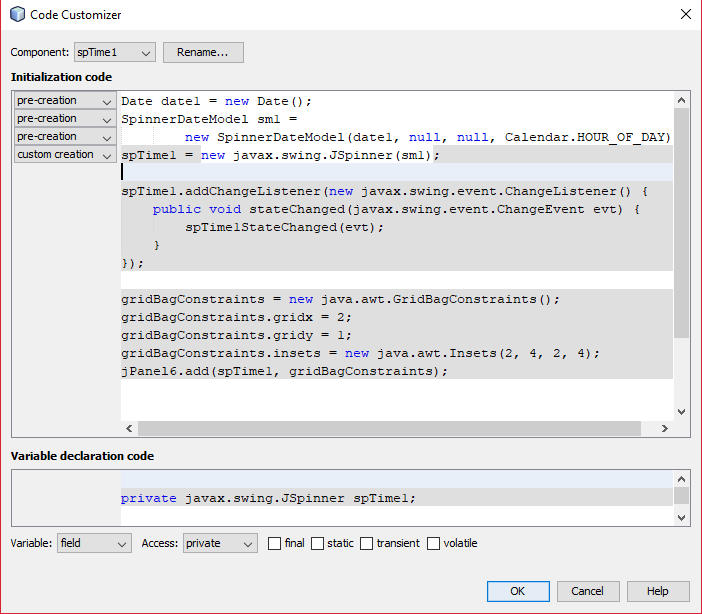
\includegraphics[width=0.70\textwidth]{Bilder/Java_Programm/SpinnerConfiguration}
  \end{center}
  \caption{Spinner Konfiguration}
  \label{SpinnerKonfiguration}
  \vspace{-20pt}
\end{wrapfigure}
\\ \\ In diesem Fenster ist der Code, welcher in den ersten vier Zeilen steht, hinzuzufügen. 
\\ Hier wird das Model für den Spinner gesetzt. Dieses Model gibt an, dass der Spinner ein Datum darstellen soll. Weiters wird nicht festgelegt was vom Datum angezeigt werden soll. Hier wird die Uhrzeit dargestellt. 
\\ \\ Diese Schritte sind für alle der vier verwendeten Spinner verwendet werden.

\vspace{30pt}

Zusätlich muss noch für jeden Spinner folgende Methode, im Constructor nach \textbf{initComponents();}, aufgerufen werden:
\begin{lstlisting}[style=Javastyle, caption=Spinner Zeitzone]
	JSpinner.DateEditor at1 = new JSpinner.DateEditor(spTime1, "HH:mm");
        	spTime1.setEditor(at1);
\end{lstlisting}

\vspace{10pt}

Im \textbf{Constructor} der \textbf{TimeManagement} Klasse werden, wenn das Fenster geöffnet wird, alle Spinner mit den momentanen Zeiten gefüllt. Zusätzlich werden noch die Häkchen, die festlegen ob eine Zeit aktiv ist, gesetzt.

\vspace{10pt}

Bevor das Fenster geschlossen wird, wenn \textbf{Abbrechen} gedrückt wird, wird überprüft, ob sich die Inhalte der Spinner verändert haben. Um dies zu überprüfen werden Events verwendet. Dafür wird für jeden Spinner das folgende Event verwendet:

\newpage

\begin{lstlisting}[style=JavaStyle, caption=Spinner Event]
    private void spTime1StateChanged(javax.swing.event.ChangeEvent evt)                                     
    {                                         
        saved = false;
    }   
\end{lstlisting} 
Diese Event wird aufgerufen, wenn der Inhalt der Spinners verwendet wird. Dabei wird dann eine Boolean-Variable, die bekannt gibt, ob etwas verwendet wurde, auf \textbf{false} gesetzt. Wenn diese Boolean-Variable auf \textbf{false} ist, wird vor dem Beenden dem Benutzer eine Warnung ausgegeben, dass noch nicht gespeichert wurde. Siehe Code-Beispiel \ref{TimeManagementSpeichern} Zusätzlich kann dann ausgewählt werden, ob wirklich ohne zu speichern beendet werden soll.

\begin{lstlisting}[style=Javastyle, caption=TimeManagement Fenster schließen, label=TimeManagementSpeichern]
 private void onCancel(java.awt.event.ActionEvent evt)                          
    {                              
       if (saved == false)
        {
            if (JOptionPane.showConfirmDialog(this, "Nicht gespeicherte Inhalte 
            	gehen verloren! Wollen Sie speichern bevor Sie das 
            	Fenster schießen?", "Hinweis", 
            	JOptionPane.YES_NO_OPTION) == JOptionPane.YES_OPTION)
            {
                getValues();
                
                dispose();
            }
        }
        else
        {
            dispose();
        }
    }
\end{lstlisting}

\vspace{10pt}

Wenn das Fenster mit \textbf{Ok} geschlossen wird, werden die Inhalte der Spinner, wenn sie geändert wurden, aus den Spinnern geholt. Zusätzlich wird das gleiche mit den ComboBoxes gemacht. Die Inhalte der Spinner und ComboBoxen werden anschließend in ein Dokument, also ein Format das für die Datenbank verständlich ist, gespeichert. Das Dokument sieht wie folgt aus:

\newpage

\begin{lstlisting}[style=Javastyle, caption=Zeitendokument]
// ... Code ...

newTimeDoc = new BasicDBObject("identifier", "Times")
                        .append("time1", time1)
                        .append("time1_active", time1_active)
                        .append("time2", time2)
                        .append("time2_active", time2_active)
                        .append("time3", time3)
                        .append("time3_active", time3_active)
                        .append("time4", time4)
                        .append("time4_active", time4_active);
\end{lstlisting}
Dieses Dokument wird anschließen mit folgender \textbf{Getter-Methode} für andere Klassen, konkret für das \textbf{MainWindow}, zugänglich gemacht:
\begin{lstlisting}[style=Javastyle, caption=Zeitendokument Getter-Methode]
public BasicDBObject getNewTimeDoc()
    {
        return newTimeDoc;
    }
\end{lstlisting}

\newpage

\subsubsection{CreateAndRegisterUser}
\begin{wrapfigure}{l}{0.6\textwidth}
\vspace{-20pt}
  \begin{center}
    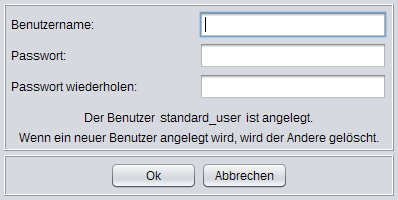
\includegraphics[width=0.60\textwidth]{Bilder/GUI/CreateUser}
  \end{center}
  \caption{CreateAndRegisterUser}
  \label{CreateAndRegisterUser}
  \vspace{0pt}
\end{wrapfigure}
Die Klasse \textbf{CreateAndRegisterUser} bietet dem Benutzer die Möglichkeit einen Benutzer anzulegen.Es ist deshalb nur ein Benutzer anlegbar, weil es bei der Anlage keinen Nutzen hätte mehrere Benutzer zu haben. Da der angelegte Benutzer nur benötigt wird sich auf der Webseite der Anlage anzumelden, ist es ausreichend nur einen Benutzer anlegen zu können. Die GUI ist in Abbildung \ref{CreateAndRegisterUser} zu sehen.
\\ \\ Die GUI der Klasse ist ein Dialogfenster. Bei Dialogfenstern ist es üblich, dass sie mit \textbf{Ok} und \textbf{Abbrechen} bedienbar sind.
\\ \\ Es ist nur möglich einen Benutzer anzulegen. Wenn bereits ein Benutzer angelegt ist und dann ein neuer angelegt wird, wird der alte Benutzer überschrieben. Um einen neuen Benutzer anzulegen müssen folgende Felder ausgefüllt werden: Benutzername, Passwort und Passwort wiederholen. Wenn eines dieser Felder leer gelassen wird, wird eine Fehlermeldung ausgegeben. Weiters wird eine Fehlermeldung ausgegeben, wenn die beiden Passwörter nicht übereinstimmen. Wenn alle drei Eingabefelder korrekt ausgefüllt wurden kann der Benutzer angelegt werden indem \textbf{Ok} gedrückt wird. Dadurch werden der Benutzer und das Passwort in das Programm übernommen und in die Datenbank gespeichert. Anschließend erscheint ein Informationsfenster welches den Benutzer darüber informiert, dass der Benutzer erfolgreich angelegt wurde. Danach schließt sich das Dialogfenster. Wenn anstatt von \textbf{Ok} \textbf{Abbrechen} gedrückt wird, schließt sich das Dialogfenster und die Änderungen werden verworfen.
\\ \\ Während das Dialogfenster geöffnet ist blockiert der EDT an der Stelle, an der das Dialogfenster geöffnet wurde.

\vspace{10pt}

Um das Passwort einzugeben wird ein \textbf{PasswordField} verwendet. Diese Eingabefeld wird speziell dazu verwendet Passwörter einzugeben. Eine Besonderheit davon ist, dass die Passwörter nicht als Text sonder als Sternchen dargestellt werden. Eine weitere ist, dass der Inhalt eine Zeichenkette ist, also ein Feld von Characters: \textbf{char[]}. Weiters unterscheidet sich auch das Abfragen des Inhaltes im Vergleich mit einem normalen Textfeld. Beim \textbf{PasswordField} kann der Inhalt mit \textbf{passwordField.getPassword()} abgefragt werden.

\newpage

Um das Passwort im Programm besser verarbeiten zu können wird es wie folgt in einen String umformatiert:
\begin{lstlisting}[style=Javastyle, caption=char zu String]
	String string_password = valueOf(char_password);
\end{lstlisting}
Beim Umformatieren des Passworts in einen String könnte ein Fehler auftreten wenn Sonderzeichen verwendet werden. Deshalb sollte verhindert werden, dass der Benutzer Sonderzeichen eingibt oder das Programm anpassen, so dass Sonderzeichen verwendet werden können.

\vspace{10pt}

Um dem Benutzer Sicherheit zu gewährleisten wird das Passwort, bevor es in der Datenbank gespeichert wird, wie folgt gehasht: 
\begin{lstlisting}[style=Javastyle, caption=Hash Passwort]
    public static String hash(String passwordToHash, String salt)
    {
        String generatedPassword = null;
        try
        {
            MessageDigest md = MessageDigest.getInstance("SHA-512");
            md.update(salt.getBytes("UTF-8"));
            byte[] bytes = md.digest(passwordToHash.getBytes(
            StandardCharsets.UTF_8));
            StringBuilder sb = new StringBuilder();
            for (int i = 0;
                    i < bytes.length;
                    i++)
            {
                sb.append(Integer.toString(
                (bytes[i] & 0xff) + 0x100, 16).substring(1));
            }
            generatedPassword = sb.toString();
        }
        catch (NoSuchAlgorithmException e)
        {
            e.printStackTrace();
        }
        catch (UnsupportedEncodingException ex)
        {
            Logger.getLogger(HashPassword.class.getName()).log(
            Level.SEVERE, null, ex);
        }
        return generatedPassword;
    }
\end{lstlisting}

Um das Password zu hashen wird der Hashalgorithmus \textbf{SHA-512} verwendet. Im Programm wird das Passwort nur einmal gehasht. Falls die Katzenfütterungsanlage in Serie gehen sollte, sollte das Passwort öfters gehasht werden um die Sicherheit zu erhöhen.
\\ Für das Hashen des Passworts wurde auf Stackoverflow \footfullcite{Stackoverflow_Hashen} recherchiert.

Mit dem Parameter \textbf{String salt} kann noch ein String übergeben werden welcher vor dem Hashen des Passworts am Passwort angehängt wird. Somit wird die Entschlüsselung des Passwort nochmals erschwert. Der  \textbf{salt} wird normalerweise als Byte-Array und nicht als String deklariert.

\vspace{10pt}

Bevor das Fenster geschlossen wird, wenn \textbf{Update} gedrückt wird, wird überprüft, ob sich die Inhalte der Text- und Passwortfelder verändert haben. Dabei wird vom Event überwacht, ob in dem Feld ein neues Zeichen eingegeben wird. Danach wird eine Boolean-Variable, die angibt ob gespeichert wurde, auf \textbf{false} gesetzt. Das Event für das Textfeld sieht wie folgt aus:
\begin{lstlisting}[style=Javastyle, caption=Textfeld Event]
	private void tfUserNameKeyPressed(java.awt.event.KeyEvent evt)                                       
	{                                           
		saved = false;
	}
\end{lstlisting}
Wenn die Variable \textbf{false} ist, also noch nicht gespeichert wurde, wird dem Benutzer die Warnung ausgegeben werden, dass die veränderten Daten noch nicht gespeichert sind.

\vspace{10pt}

Wenn das Dialogfenster mit \textbf{Ok} bestätigt wird, wird das Benutzername und das Passwort in ein Dokument, welches für die Datenbank verständlich ist, gespeichert. Dieses Dokument sieht wie folgt aus:
\begin{lstlisting}[style=Javastyle, caption=Benutzerdokument]
newUserDoc = new BasicDBObject("identifier", "User").append("user_name", 
	user_name).append("user_password", hashedPassword);
\end{lstlisting}

Dieses Dokument wird anschließend noch mit einer \textbf{Getter-Methode} für das  \textbf{MainWindow} zugänglich gemacht:
\begin{lstlisting}[style=Javastyle, caption=Benutzerdokument Getter-Methode]
	public BasicDBObject getNewUserDoc()
	{
		return newUserDoc;
	}
\end{lstlisting}

\subsubsection{ManualControl}
  \begin{figure}[H]
    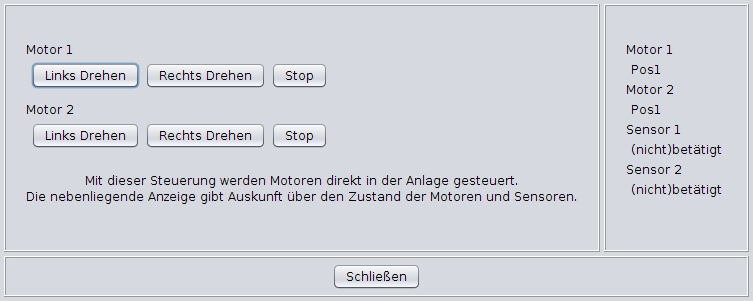
\includegraphics[width=0.90\textwidth]{Bilder/GUI/ManualControl}
    \caption{ManualControl}
  \label{ManualControl}
  \end{figure}
In der Klasse \textbf{ManualControl} wird eine manuelle Steuerung für die Motoren implementiert. Dies erleichtert dem Benutzer das Reinigen der Anlage, weil er zum Beispiel die Drehplatte, mit den Futterschüsseln, immer nachdrehen kann. Das gleiche gilt für das Förderband.
\\ Das GUI Fenster ist in Abbildung \ref{ManualControl} zu sehen.
\\ Die GUI der Klasse ist ein Steuerfenster. Da dieses Fenster ein Steuer- und kein Dialogfenster ist, werden kein \textbf{Ok} und \textbf{Abbrechen} benötigt. Aus diesem Grund ist nur ein Knopf \textbf{Schließen} vorhanden.

\vspace{10pt}

Wie beim Dialogfenster blockiert das Steuerfenster den EDT der Stelle wo es geöffnet wurde bis es wieder geschlossen wird.

\vspace{10pt}

Dieses Fenster ist aus Sicherheitsgründen nur dann aufrufbar, wenn der Maschinenzustand auf Aus ist. Der Grund dafür ist, dass es zu Fehlern kommen kann, wenn während einer Fütterung ein Motor ein oder aus geschalten wird.
\\ Weiters wird der Benutzer bevor er dieses Steuerfenster öffnet darüber informiert, dass er nun direkt die Motoren steuert. Zusätzlich wird der Benutzer gefragt, ob er die Steuerung wirklich öffnen will.
\\ Der Benutzer kann nun beide Motoren unabhänging voneinander steuern. Er kann die Motoren in und gegen den Uhrzeigersinn drehen. Dazu muss er den Knopf mit der jeweiligen Drehrichtung im Steuerungsfenster klicken. Die Motoren sind mit dem jeweiligen Stop-Knopf wieder stopbar.
\\ Falls die Motoren vom Benutzer vor dem Schließen des Fensters nicht gestoppt werden, werden diese automatisch vom Programm gestopt. Dies dient dazu, dass sichergestellt ist, dass die Motoren immer gestoppt werden.
\\ Die Methode zum Schließen des Fensters, welche auch die Motoren stoppt, sieht wie folgt aus:

\newpage

\begin{lstlisting}[style=JavaStyle, caption=Motoren stoppen und Fenster schließen]
	private void onClose(java.awt.event.ActionEvent evt)                                
    	{                                 
       		// stop engines when closing the conrtol dialog
       		// security measurement
       		
        	pi4jInstance.stopEngine1();
        	pi4jInstance.stopEngine2();
        
        	dispose();
    	} 
\end{lstlisting}

\vspace{10pt}

Neben dem Bereich für die Steuerung befindet sich noch ein Bereich in dem die Echtzeit-Zustände aller Motoren und Sensoren angezeigt werden. So kann der Benutzer, ohne direkt in die Anlage sehen zu müssen, feststellen, ob sich ein Motor dreht oder ein Sensor betätigt ist.

\vspace{10pt}

Die Motoren werden gesteuert, indem beim Drücken eines Knopfes, eine Methode aus dem \textbf{pi4j Singleton} (Kaptiel \ref{subsec:pi4j}) aufgerufen wird. Das Singleton-Objekt steuert in weiterer Folge die Output-Pins.
\\ Wenn ein Knopf gedrückt wird, wird die jeweilige zum Knopf gehörente Methode aufgerufen. Dies kann wie folt aussehen:
\begin{lstlisting}[style=JavaStyle, caption=Motoren drehen] 
	private void onMoveEngine1Counterclockwise(java.awt.event.ActionEvent evt)                                               
    	{                                                   
        	pi4jInstance.moveEngine1Counterclockwise();
    	}  
\end{lstlisting}

\vspace{10pt}

Um die aktuellen Positionen der Motoren und Zustände der Sensoren zu ermitteln und auszugeben wird ein SwingWorker verwendet. Dies ist unter Kapitel \ref{subsubsec:Positionsinformation} genauer beschrieben.

\newpage

\subsubsection{Positionsinformation} \label{subsubsec:Positionsinformation}
\begin{wrapfigure}{l}{0.25\textwidth}
\vspace{-20pt}
  \begin{center}
    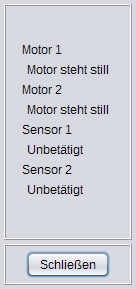
\includegraphics[width=0.25\textwidth]{Bilder/GUI/Positionsinformation}
  \end{center}
  \caption{Positionsinformation}
  \label{Positionsinformation}
  \vspace{-10pt}
\end{wrapfigure}
In der Klasse \textbf{Positionsinformation} wird dem Benutzer eine Übersicht über die Zustände der Motoren und Sensoren geboten. So kann er ohne, direkt in die Anlage zu sehen, feststellen, ob sich ein Motor dreht oder ein Sensor betätigt ist.
\\ Die GUI ist in Abbildung \ref{Positionsinformation} zu sehen.
\\ Die GUI der Klasse ist ein Informationsfenster. Da dieses Fenster kein Dialogfenster ist, werden \textbf{Ok} und \textbf{Abbrechen} nicht benötigt. Aus diesem Grund reicht ein Knopf \textbf{Schließen} aus.

\vspace{10pt}

Wie beim Dialogfenster blockiert das Informationsfenster den EDT, an der Stelle wo es geöffnet wurde, bis es wieder geschlossen wird.

\vspace{10pt}

Dieses Fenster ist, im Gegensatz zu \textbf{ManualControl}, auch aufrufbar, wenn die Fütterung aktiviert, also der Maschinenzustand auf \textbf{Ein}, ist.
\\ Bei der Anzeige für Drehrichtung der Motoren und die Zustände der Sensoren kann folgendes angezeigt werden:
\begin{itemize}
\item[1] Motoren
  \begin{itemize}
    \item[•] Motor steht still
    \item[•] Motor dreht links
    \item[•] Motor dreht rechts
  \end{itemize}
\item[2] Sensoren
  \begin{itemize}
    \item[•] Unbetätigt 
    \item[•] Betätigt 
  \end{itemize}
\end{itemize}

\vspace{10pt}

Die Drehrichtungen und die Zustände werden mithilfe des \textbf{pi4j Singleton} (Kapitel \ref{subsec:pi4j}) erfasst. In dieser Klasse sind Methoden implementiert, die diese Messungen durchführen können.
\\ Um dies annähernd echtzeitfähig zu realisieren wird ein SwingWorker verwendet. Im \textbf{doInBackground()} dieses SwingWorkers, siehe Code-Beispiel \ref{SwingWorker_MotorSensorStatus}, werden die Zustände der Motoren und Sensoren abgefragt. Diese Zustände werden mit einem \textbf{publish()} an ein \textbf{process()} übergeben. Im \textbf{process()} werden die Zustände in die Label der GUI geschrieben.
\\ Das \textbf{process()} sieht wie folgt aus:

\newpage

\begin{lstlisting}[style=JavaStyle, caption= Label aktualisieren]
	@Override
    protected void process(List<String[]> chunks)
    {
         String state[] = chunks.get((chunks.size() - 1));
            
         lbSensor1.setText(state[0]);
         lbSensor2.setText(state[1]);
         lbEngine1.setText(state[2]);
         lbEngine2.setText(state[3]);
    } 
\end{lstlisting}
Das \textbf{doInBackground()} ist wie folgt implementiert:
\begin{lstlisting}[style=JavaStyle, caption= Motor- und Sensorzustände, label=SwingWorker_MotorSensorStatus]
	@Override
        protected Object doInBackground() throws Exception
        {                        
            while (!isCancelled())
            {
                strSensor1 = pi4j_instance.statusSensor1();
                strSensor2 = pi4j_instance.statusSensor2();
                strEngine1 = pi4j_instance.statusEngine1();
                strEngine2 = pi4j_instance.statusEngine2();
                
                String state[] = null;
                state[0] = strSensor1;
                state[1] = strSensor2;
                state[2] = strEngine1;
                state[3] = strEngine2;
                
                publish(state);
                
                TimeUnit.MILLISECONDS.sleep(100);
            } 
            return 1;            
        }

\end{lstlisting}
In diesem \textbf{doInBackground()} werde  alle 100 Millisekunden die Motordrehrichtungen und die Sensorzustände abgefragt. Somit ist das nur eine annähernd echtzeitfähige Abfrage der Zustände. Dies wird so realisiert um die Prozessorauslastung zu verringern.

\newpage

\subsubsection{SystemInfo}
\begin{wrapfigure}{l}{0.40\textwidth}
\vspace{-20pt}
  \begin{center}
    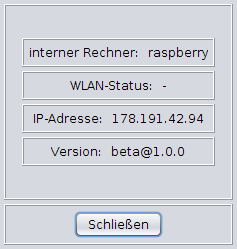
\includegraphics[width=0.40\textwidth]{Bilder/GUI/SystemInfo}
  \end{center}
  \caption{SystemInfo}
  \label{SystemInfo}
  \vspace{-60pt}
\end{wrapfigure}
   
In der Klasse \textbf{SystemInfo} werden dem Benutzer wichtige Informationen über seine Anlage angezeigt. Das GUI Fenster ist ein Informationsfenster. Das Fenster blockiert den EDT, an der Stelle an der es geöffnet wird, bis es geschlossen wird. Da dies nur ein Informationsfenster ist reicht ein Knopf \textbf{Schließen} für die Bedienung aus.

\vspace{10pt}

\begin{comment}
Die Seriennummer dient dazu eine Anlage eindeutig zu identifizieren. Die Seriennummer wird jeder Anlage durch einen Server gegeben. Dieser Server enthält einen Zähler, welcher nach jeder vergebenen Nummer \textbf{+1} nach oben zählt. Die Seriennummer wird anschließend in der Datenbank am Raspberry gespeichert. Das abfragen der Seriennummer aus der Datenbank erfolgt wie folgt:

\vspace{40pt}
\begin{lstlisting}[style=JavaStyle, caption=Abfragen der Seriennummer]
	infoDoc = MainWindow.getInstance().getInfoDoc();
	strInfo = JSON.serialize(infoDoc);

	jsonReader = Json.createReader(new StringReader(ipJson));
    JsonObject ipObj = jsonReader.readObject();
    jsonReader.close();
        
    ip = ipObj.getString("ip");        
\end{lstlisting}
Bei diesem Code-Beispiel wird zu Beginn, die Collection in der die benötigten Informationen gespeichert sind, aus der Datenbank geladen. Anschließend werden die Daten in einen \textbf{String} und dann weiter in ein \textbf{JsonObject} umgewandelt. Danach kann die Seriennummer als \textbf{Integer-Zahl} aus dem \textbf{JsonObject} gelesen werden. Diese Zahl wird dann in einen \textbf{String} umgewandelt um in der GUI ausgegeben werden zu können.
\end{comment}

\vspace{10pt}

Der Name, des in der Anlage verbaute Rechners, wird in der Datenbank eingelesen. Dies funktioniert indem die aus der Datenbank gelesenen Dateien von einem String in ein JsonObject umgewandelt werden. Anschließend kann aus dem JsonObject dar Name des verbauten Rechners ausgelesen werden.

\vspace{50pt}

Der WLAN-Status wird wie der Name des internen Rechners aus der Datenbank eingelesen. Der WLAN-Status wird in die Datenbank geschrieben, wenn sich der Raspberry mit einem WLAN verbindet. \textbf{(ref zu Greisls schriftlichen Teil sobald es geschrieben} wurde)

\vspace{10pt}

Die IP-Adresse der Anlage wird vom Web-Server geholt, welcher diese ermittelt. Dieser Server läuft ebenfalls am Raspberry und ist immer unter einem festgelegtem Port aktiv. Die IP-Adresse wird wie folgt, im \textbf{MainWindow}, abgefragt:
\begin{lstlisting}[style=JavaStyle, caption=Abfragen der IP-Adresse]
	URL urlIp = new URL("http://localhost:17325/api/ip");
	
	URLConnection conIp = urlIp.openConnection();
	
	BufferedReader bReaderIp = new BufferedReader(
	new InputStreamReader(conIp.getInputStream()));    
	
	final StringBuilder sbIp = new StringBuilder();
	
	while ((line = bReaderIp.readLine()) != null)
	{
		sbIp.append(line);
	}
            
	ip = sbIp.toString();    
\end{lstlisting}
In diesem Code-Beispiel wird zuerst die URL, unter der der Server zu erreichen ist, festgelegt. Anschließend wird eine Verbindung mit der Server aufgebaut. Wenn die Verbindung besteht wird ein \textbf{BufferdReader} und ein \textbf{StringBuilder} erstellt. Der \textbf{BufferdReader} dient dazu, um die IP-Adresse vom Server zu lesen. Der \textbf{StringBuilder} wird benötigt um den String zusammenzufügen, wenn mehrere Zeilen eingelesen werden müssen. Zum Schluss wird mit \textbf{sbIp.toString()} der String erstellt, welcher mit einer GETTER-Methode für die Klasse \textbf{SystemInfo} zugänglich gemacht wird.

\vspace{10pt}

Die Version wird sowie die IP-Adresse von einem Server abgefragt. Das Abfragen wird nach dem gleichen Schema wie bei der IP-Adresse im \textbf{MainWindow} gemacht. Der erstellte String wird auch hier mit einer GETTER-Methode für die Klasse \textbf{SystemInfo} zugänglich gemacht.


\newpage

\subsubsection{Update}\label{subsubsec:Update}
\begin{figure}[H]
  \begin{minipage}[hbt]{0.45\textwidth}
    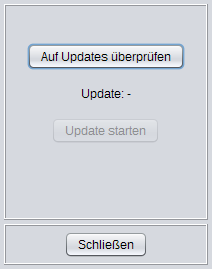
\includegraphics[width=0.9\textwidth]{Bilder/GUI/Update1}
 	\caption{Update suchen}
  	\label{Update}
  \end{minipage}
\hspace{.03\linewidth}
  \begin{minipage}[hbt]{0.45\textwidth}
    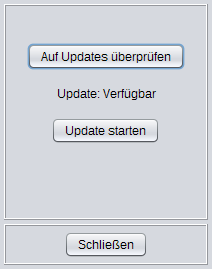
\includegraphics[width=0.9\textwidth]{Bilder/GUI/Update2}
  	\caption{Update verfügbar}
  	\label{Update2}
  \end{minipage}
  \vspace{0pt}
\end{figure}
Mit der \textbf{Update} Klasse ist es dem Benutzer möglich die Software seiner Anlage aktuell zu halten. Die GUI der Klasse ist auch ein Steuerfenster. Deswegen werden kein \textbf{Ok} und \textbf{Abbrechen} benötigt und es kann ein Knopf \textbf{Schließen} verwendet werden. Während einem Update ist der \textbf{Schließen} Knopf nicht verfügbar.

\vspace{10pt}

Wie beim Dialogfenster blockiert das Steuerfenster den EDT an der Stelle wo es geöffnet wurde bis es wieder geschlossen wird.

\vspace{10pt}

Wenn das Fenster aufgerufen wird, hat es das Aussehen aus der Abbildung \ref{Update}. Nun kann der Benutzer das Fenster schließen oder den Knopf \textbf{Auf Updates überprüfen} drücken. Sofern ein Update gefunden wird, wird der Knopf \textbf{Update starten} aktiviert und das Label ändert sich von \textbf{-} auf \textbf{Verfügbar}. Also sieht das Fenster aus wie in Abbildung \ref{Update2}.

\vspace{10pt}

Beim Überprüfen auf Updates wird die lokale Versionsnummer am Raspberry mit der globalen Versionsnummer am Git-Repository verglichen. Wenn die Versionen nicht übereinstimmen ist ein Update verfügbar. Obwohl die Versionsnummer immer chronologisch nach oben gezählt wird, wird auch ein Update gemacht wenn die Versionsnummer niedriger wird. Der Grund dafür ist, wenn eine Version einmal einen schwerwiegenden Fehler beinhaltet, ist es ohne Probleme möglich auf die vorherige Version zurück zu gehen. 

\vspace{10pt}

Die Daten für das Update werden von einem Git-Repository herunter geladen. Dies wird mit einem \textbf{git pull} Befehl gemacht. Anschließend wird am Raspberry eine Datei bearbeitet, welche dem Raspberry beim Startet mitteilt, dass die Programme neu zu bauen sind. Nach jedem Update wird das Raspberry automatisch neu gestartet.

\vspace{10pt}

Wenn nun der Knopf \textbf{Update starten} gedrückt wird, wird folgende Methode aufgerufen:
\begin{lstlisting}[style=JavaStyle, caption= Update]
    private void onUpdate(java.awt.event.ActionEvent evt)                          
    {                              
        try
        {
            btClose.setEnabled(false);
            
            Process process = Runtime.getRuntime().exec("git pull");
            process.waitFor();

            write();

            pTextUpdateErfolgreich.setVisible(true);
            btClose.setEnabled(true);

            Runtime.getRuntime().exec("sudo reboot");

        }
        catch (IOException ex)
        {
            Logger.getLogger(Update.class.getName()).log(Level.SEVERE, null, ex);
        }
        catch (InterruptedException ex)
        {
            Logger.getLogger(Update.class.getName()).log(Level.SEVERE, null, 
            "WaitFor ist interrupted");
        }        
    }
\end{lstlisting}

\newpage

\begin{lstlisting}[style=JavaStyle, caption= Writer]
    private void write()
    {
        String path = String.format(
        "/home/" + System.getProperty("user.name") + "/git/fuettr/build");

        try (final BufferedWriter writer
                = new BufferedWriter(
                        new OutputStreamWriter(
                                new FileOutputStream(path), "utf8"));)
        {
            writer.write(String.format("true"));
        }
        catch (Exception ex)
        {
            ex.printStackTrace();
        }
    }
\end{lstlisting}
Der Pfad, der zum Speicherort der Datei führt, beinhaltet den Benutzernamen des Raspberrys. Deswegen wird die Methode \textbf{\inlinecode{JavaStyle}{System.getProperty("user.name")}} verwendet, um den aktuellen Benutzernamen herauszufinden.

\vspace{10pt}

Wenn das Update, zum Beispiel durch einen Stromausfall, unterbrochen wird, sollte das kein Problem darstellen. Sofern der Stromausfall während dem Downloaden eintritt, wird am Raspberry nichts verändert, weil das Neubauen der Programme erst beim Neustarten des Raspberrys gemacht wird. Wenn nun der Download unterbrochen wird, wird die Datei, die dem Raspberry mitteilt, dass die Programme neu zu bauen sind, nicht bearbeitet. Nach dem Stromausfall kann das Raspberry normal gestartet werden und das Update kann neu gestartet werden.

\newpage

\section{Zusammenfassung - Verbesserungsmöglichkeiten - Probleme}

\subsection{Probleme}
\subsubsection{Problem mit Mongodb am Raspberry}
Mit Mongodb gab es ein Problem am Raspberry. Die neueren Versionen werden nämlich nicht unterstützt. Aus diesem Grund musste auf die älteste erhältliche Version 2.14.2 zurückgegriffen werden.
\\ Es gibt auch Möglichkeiten die neuen Versionen am Raspberry verwenden zu können. Diese Lösungen sind im Rahmen einer Diplomarbeit zu zeitintensiv.
\\ Wenn das Projekt weiter geführt werden sollte, sollte überprüft werden, ob die neueste Version von Mongodb mit dem Raspberry kompatibel ist.
\subsubsection{Probleme mit pi4j}
Mit der pi4j Version 1.1 ist das Problem aufgetreten, dass am Raspberry Pi 3 die IO-Pins nicht gefunden wurden. Um sicherzugehen, dass der Fehler nicht im Programm liegt wurde das Code-Beispiel von pi4j verwendet. Auch beim Testen mit diesem Code trat der Fehler, dass die IO-Pins nicht gefunden werden können, auf.
\\ Dieses Problem wurde mit dem verwenden von der pi4j Version 1.2 Snapshot gelöst. Mit der Snapshotversion werden nun alle Pins gefunden
\\ Wenn dieses Projekt weiter fortgeführt wird, sollte überprüft werden, ob von der Snapshotversion auf eine Betaversion gewechselt werden kann.

\subsection{Verbesserungsmöglichkeiten}
\subsubsection{GUI auf "Touchscreen-Design\grqq{} abändern}
Die GUI, die momentan bei der Anlage in Verwendung ist, ist nicht optimal um über einen Touchscreen-Display bedient zu werden.
\\ Dabei sollte vor allem die Navigation überarbeitet werden: 
\\Für die Navigation sollte keine Menüleiste verwendet werden. Es wäre besser, wenn Pfeile verwendet werden, um zwischen den Fenstern zu wechseln. Eine andere Möglichkeit wäre, wenn die Fenster über eigene Icons im Hauptfenster aufrufbar wären.
\subsubsection{Bessere Benutzerverwaltung - Mehrere Benutzer anlegen}
Es könnte eine Möglichkeit geschaffen werden, mehrere Benutzer anzulegen. Dadurch wäre es möglich, Benutzer zu speichern, obwohl momentan ein anderer Benutzer eingeloggt ist. Dazu muss die GUI zum verwalten der Benutzer auch abgeändert werden. Zuerst muss unterschieden werden, ob ein Benutzer angelegt werden soll oder ob man sich mit einem Benutzer auf der Anlage anmelden will. Weiters könnte noch eine Übersicht über alle, an der Anlage angelegten Benutzer, hinzugefügt werden.
\subsubsection{Selbst erstellbare Vorlagen in denen Zeiten gespeichert werden}
Die Bedienung könnte dem Benutzer erleichtert werden, wenn er bereits bestehende oder selbst erstellte Vorlagen verwenden könnte. In diesen Vorlagen könnten die Fütterungszeiten und ob diese aktiv sind gespeichert werden. Diese Profile werden zusammen mit dem Benutzernamen auf einem Server abgespeichert. Daraus folgt, dass dem Benutzer, wenn er die Anlage wechselt und er sich erneut anmeldet, wieder alle Vorlagen zur Verfügung stehen. Dann kann er eine Vorlage auswählen und muss nicht alle Zeiten manuell einstellen.

\subsection{Zusammenfassung}
Bei der Umsetzung hat es, abgesehen von den oben angeführten, keine weiteren Probleme gegeben. Der Zeitplan wurde nicht ganz eingehalten. Dabei wurden öfters die Reihenfolge der Arbeitsschritte verändert. Terminlich gibt es keine große Verzögerung.